
\chapter{Experimental evaluation: the SHO alignment problem \label{chap:Experimental-evaluation-the-SHO-alignment-problem}}

% First paragraph has no indentation.

\noindent This chapter introduces a static network simulator to find
downlink and uplink SHO areas. By introducing a penalty-based objective
function and some hard constraints, we formally define the problem
of balancing SHO areas in UMTS networks. The state-of-the-art mathematical
model used and the penalty scores of the objective function are set
according to the configuration and layout of a real mobile network,
deployed in Slovenia by Telekom Slovenije, d.d.. The balancing problem
is then tackled by three optimization algorithms, each of them belonging
to a different category of metaheuristics. We report and analyze the
optimization results, as well as the performance of each of the optimization
algorithms used.


\section{Introduction and motivation \label{sec:Introduction}}

In mobile networks, handover is one of the main features that allows
user's mobility \cite{WCDMAforUMTS_RadioAccessForThirdGenerationMobileCommunications}.
The concept behind the handover operation is simple: when a user moves
from the coverage area of a cell to the coverage area of a neighboring
cell, the system creates a new connection with the latter cell and
disconnects the user from the former one, while keeping the current
connection active. Soft-handover (SHO), on the other hand, is a possibility
available in mobile networks using the Wideband Code Division Multiple
Access (WCDMA) technology, which the Universal Mobile Telecommunications
System (UMTS) employs. SHO enhances handover functionality by allowing
a user to potentially operate on multiple radio links in parallel.
Since different users are separated by unique spreading codes, the
detection of single user's signal is implemented by despreading with
the same code sequence used in the transmitter \cite{WCDMAforUMTS_RadioAccessForThirdGenerationMobileCommunications}.

Every mobile terminal constantly monitors the common pilot power channel
(CPICH) of the connected cell and its neighbors. The information about
these measurements is sent to the network by the user terminal (i.e.
mobile). The SHO condition depends on the relative received signal
quality from different cells and the SHO window, which triggers the
addition of a cell to the user's active set. Depending on radio propagation
characteristics and different transceiver capabilities, the radio
transmission can gain more than 3 dB out of a SHO situation \cite{WCDMAforUMTS_RadioAccessForThirdGenerationMobileCommunications}.
From this point of view, SHO is a method to reduce interference and
improve radio quality, particularly at the cell border where radio
coverage is of inferior quality. In UMTS Release 99 \cite{3GPP_R99},
SHO is specified to work from the network towards the user (i.e. downlink),
and from the user towards the network (i.e. uplink).

With the introduction of High Speed Packet Access (HSPA) as an improvement
of the performance existing in WCDMA protocols, the role SHO plays
in mobile network configuration and functioning slightly changed.
The key difference is that High Speed Downlink Packet Access (HSDPA)
does not support SHO, while the High Speed Uplink Packet Access (HSUPA)
does. This particular distinction has some key implications in the
balanced distribution of SHO areas, and thus in the quality of HSPA
services \cite{holma2006hsdpa}.



\begin{figure*}[tp]
\centering

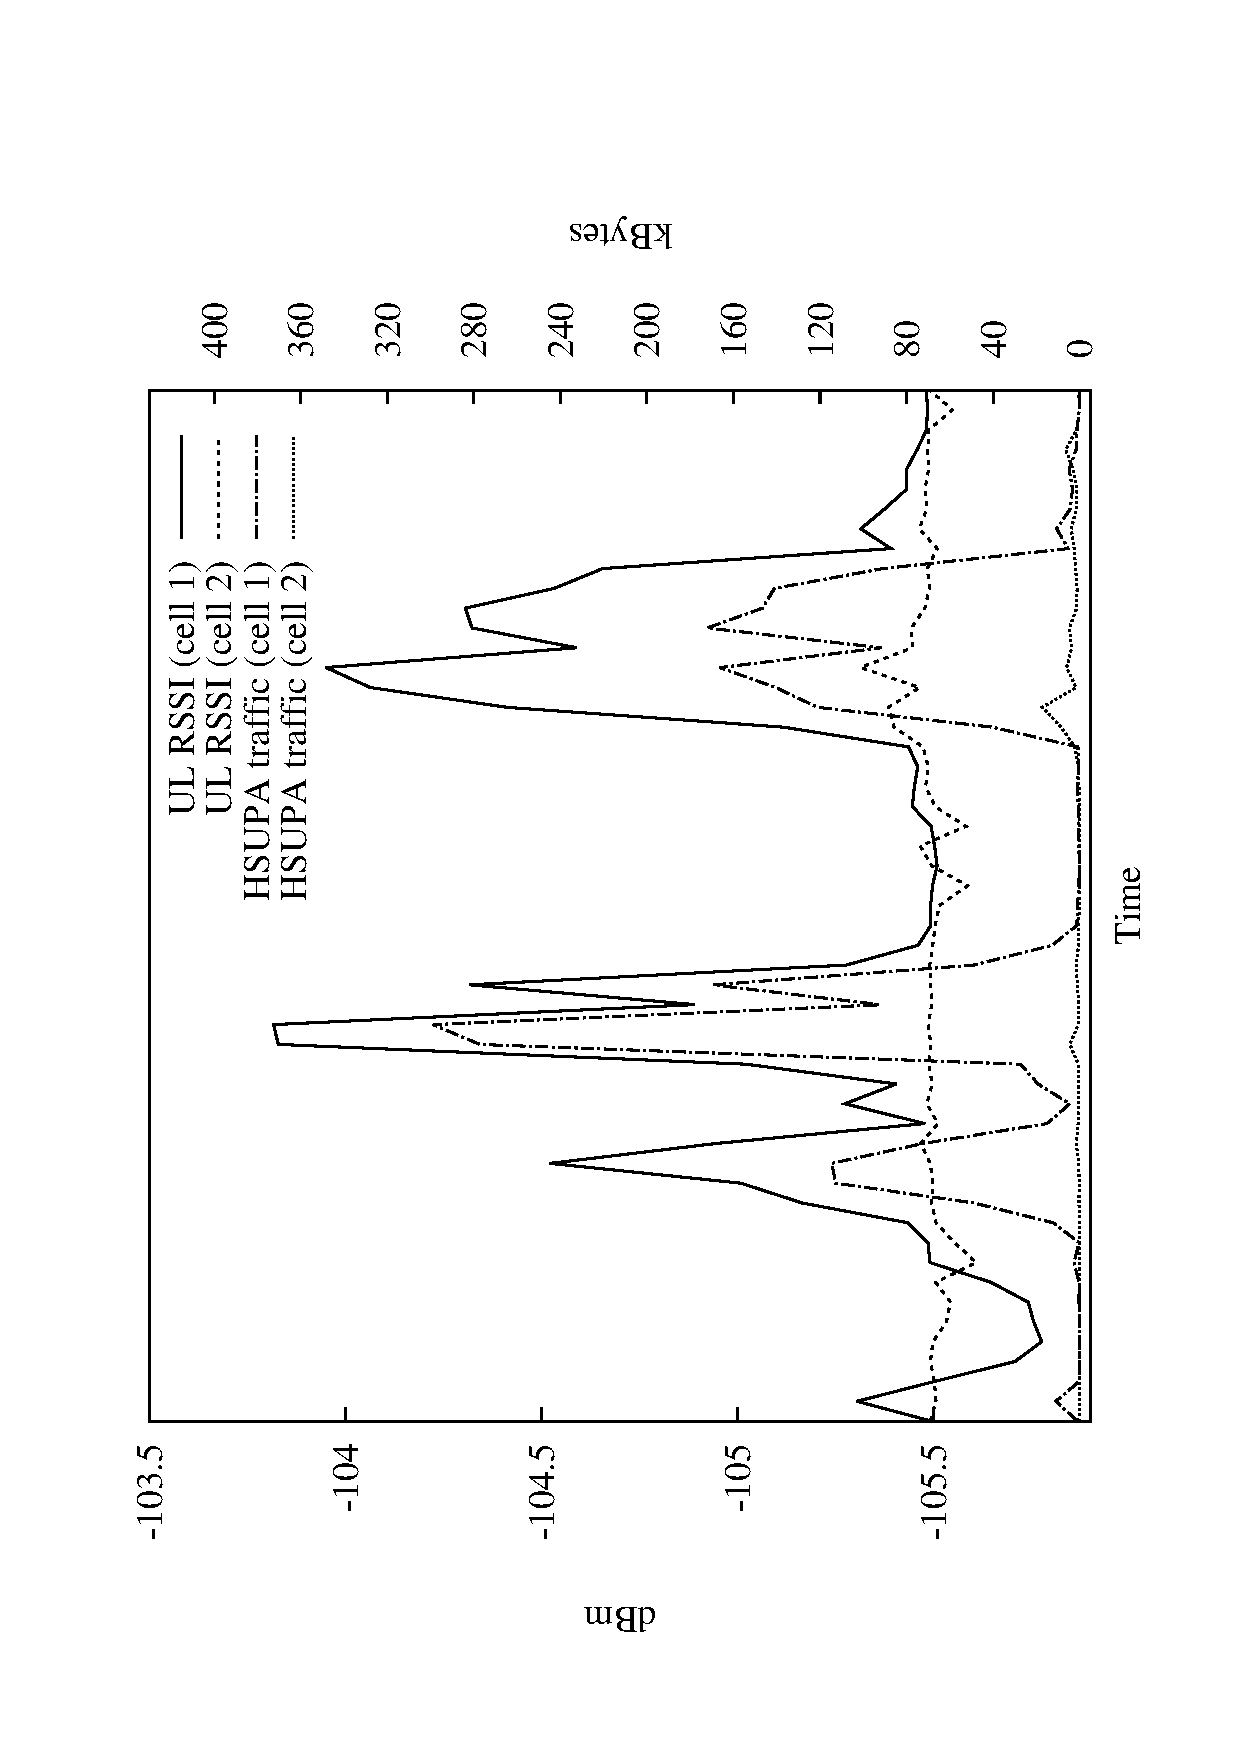
\includegraphics[width=3.7in]{07-experimental_evaluation/img/network_normal}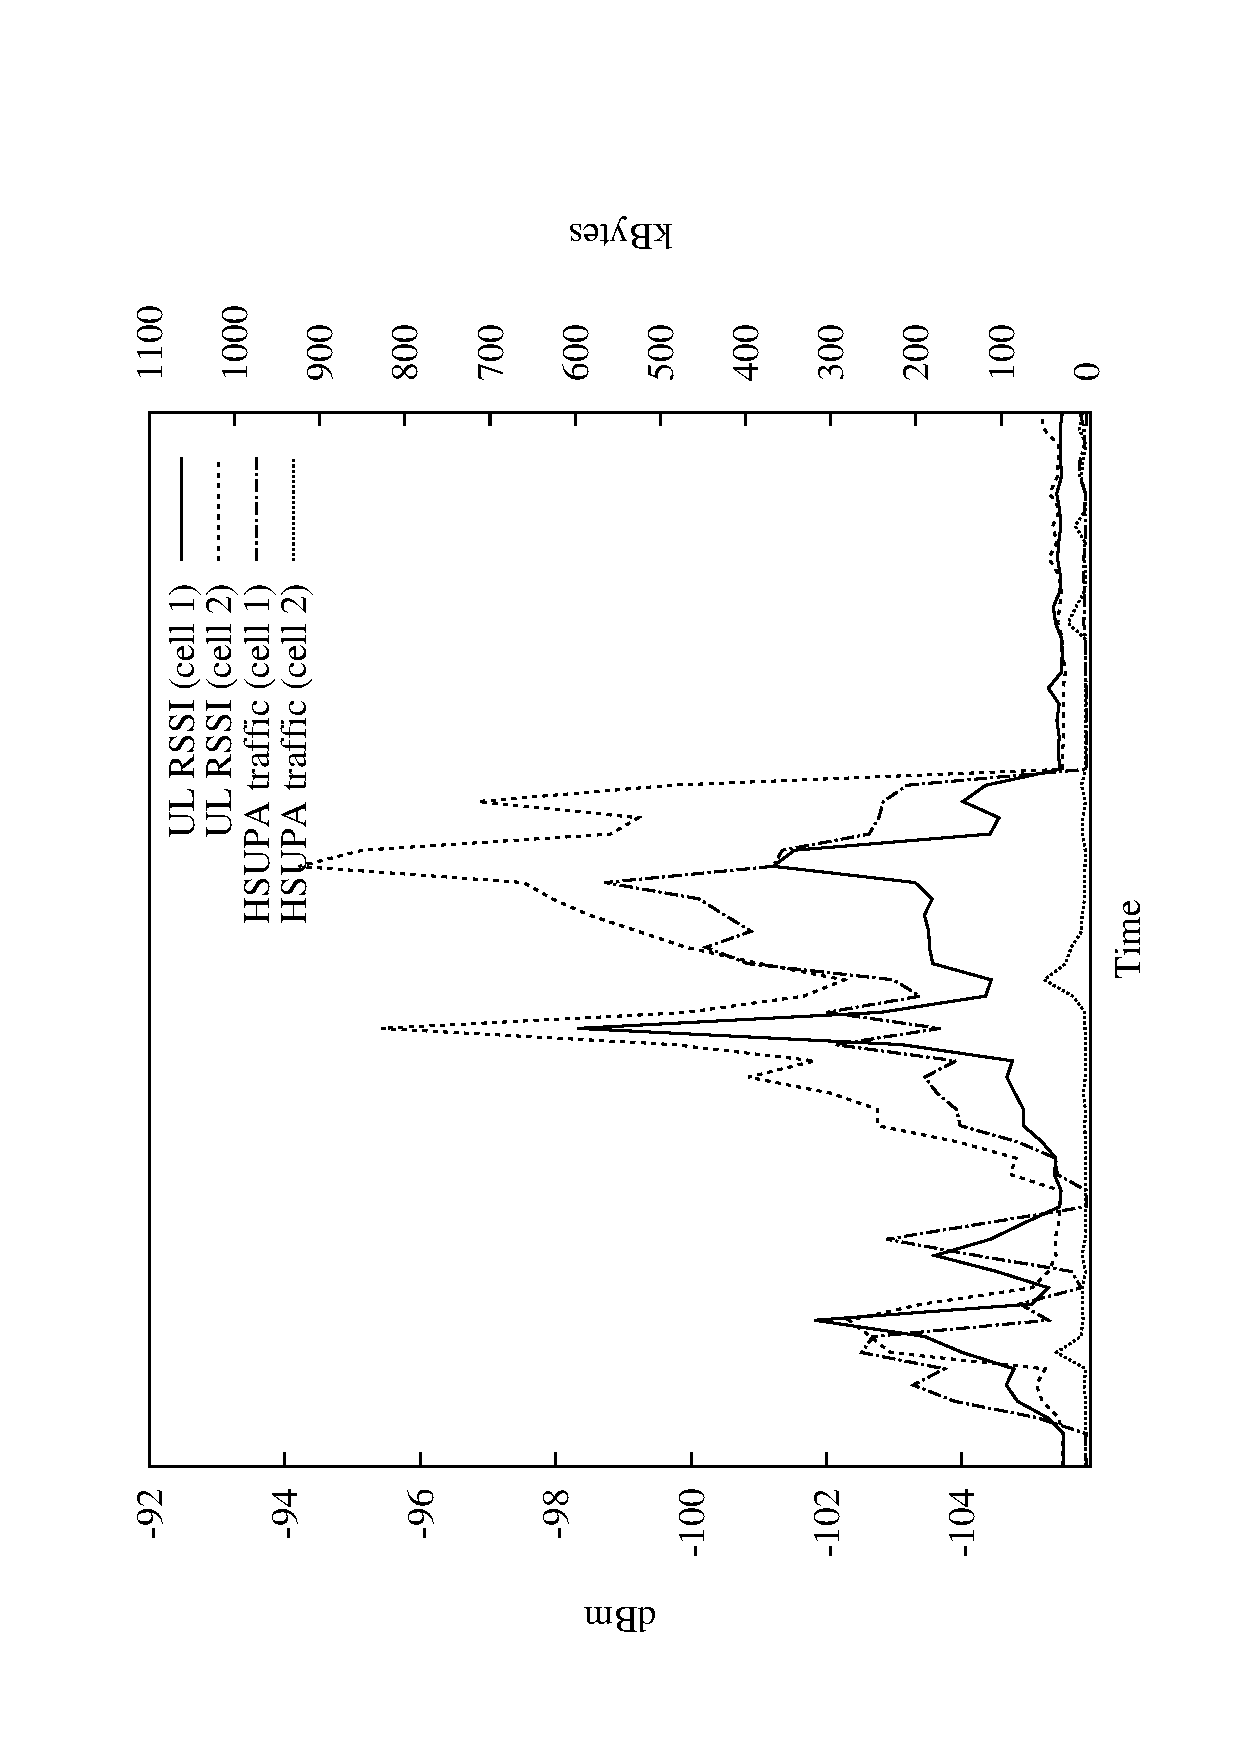
\includegraphics[width=3.7in]{07-experimental_evaluation/img/network_problem}\\\vskip -0.3in(a)\hspace*{3.6in}(b)

\caption{HSUPA traffic and uplink interference with: (a) balanced downlink
and uplink SHO conditions; (b) unbalanced downlink and uplink SHO
conditions.\label{fig:problem_illustration}}
\end{figure*}


Despite several built-in mechanisms that allow the network to overcome
different problems due to the lack of SHO during a HSDPA connection,
some abnormal cases do arise, especially in those areas where there
is SHO capability in the uplink, but none in the downlink. An example
of such a case is depicted in Figure \ref{fig:problem_illustration},
which shows interference behavior during a HSPA connection in normal
SHO conditions (a), and in unbalanced SHO conditions (b). Graph data
are actual radio network statistics, taken from the mobile network
deployed in Slovenia by Telekom Slovenije, d.d.. The graph on the
left (a) shows a normal HSUPA-enabled service situation, in which
the measured interference is proportional to the traffic being served.
Note how the noise rises with the increased traffic on cell 1, while
its neighbor (cell 2) has almost no interference nor traffic. Moreover,
the graph profile for both traffic and noise of cell 1 are almost
identical. The graph on the right (b) depicts a problematic situation,
where the noise level does not only rise on the cell serving the HSUPA
services (cell 1), but also on the neighboring one. Notice how the
interference level rises on the cell that has almost no traffic (cell
2). It is clear that the source of this noise rise is generated by
the active connection on cell 1, which shows an increase in HSUPA
traffic. However, the noise level profile on cell 2 does not follow
its traffic, as it did in the normal situation (a). This is due to
cell 2 not being part of the active set. Such situations appear when
the UL coverage is larger than the DL coverage. Interestingly enough,
this seems to be an exceptional case, as Holma and Toskala write in
\cite{holma2006hsdpa} when describing soft handover in Chapter 5:

''... There is no obvious reason why the serving E-DCH cell would
not be the same as the serving HSDPA cell, and this is also required
to be the case in the specifications.''

Given the described context, the challenge is to achieve the correct
balance or distribution of downlink and uplink SHO areas within a
working UMTS network. Therefore, the network has to be fine-tuned
to achieve a better SHO-area balancing, and thus avoiding the appearance
of problematic situations as shown in Figure \ref{fig:problem_illustration}.
This clearly implies that the mobile network configuration should
not be excessively altered, since other aspects of the network are
working well before starting the optimization process. Hence, we have
decided to define an optimization problem which objective is to find
a CPICH power level configuration for all the cells in the working
network, such that the balance of downlink and uplink SHO areas is
improved and other network aspects are preserved. The optimization
process takes into account different kinds of hardware (e.g. amplifiers,
cables, and antennas), but only the CPICH powers of the cells are
to be changed.

In this paper we utilize a static network simulator, based on a state-of-the-art
mathematical model \cite{nawrocki2006understanding}, to find downlink
and uplink SHO areas. By introducing a penalty-based objective function
and some hard constraints, we formally define the problem of balancing
SHO areas in UMTS networks. The mathematical model and the penalty
scores of the objective function are set according to the configuration
and layout of a real mobile network, deployed in Slovenia by Telekom
Slovenije, d.d.. The SHO settings are also taken from actual network
configuration, still they were adapted to closely model interference
and other dynamics present in the network. The balancing problem is
then tackled by three optimization algorithms, each of them belonging
to a different category of metaheuristics. The optimization results,
as well as the performance of each of the optimization algorithms
used, are afterwards analyzed.

The remainder of this paper is organized as follows: in Section \ref{sec:Related-work-1}
we give an overview of other works related to CPICH-power and SHO
optimization in UMTS. The static network model is presented in Section
\ref{sec:Static_network_model}, where all the elements of the mathematical
model and the objective function are defined. In Section \ref{sec:Optimization-algorithms}
we introduce and shortly describe the optimization algorithms used
to tackle the balancing problem. The simulations, including their
environment and parameter setup, are described in Section \ref{sec:Simulations-1},
followed by their results in Section \ref{sec:Results}. We conclude
with Section \ref{sec:Conclusion} by giving a conclusion and guides
for future work.




\section{Related work \label{sec:Related-work-1}}

SHO optimization has received quite some attention from the scientific
community in the last years. This mainly relates to the importance
it has within deployed networks that provide high speed services such
as video telephony \cite{chen2010_impact_of_soft_handover} and Internet
access by means of HSPA \cite{chen2011_coverage_planning_for_optimizing_HSDPA}.

Some authors tackle optimization problems at the planning stage of
the network \cite{Eisenblatter_OptimizationMethodsForUMTSRadioNetworkPlanning,ghosh2011_optimising_CDMA_cell_planning},
considering, among other variables, base station locations and hardware.
The fact is that most mobile operators are unable to apply these contributions
to a live network since the planning phase has long been concluded.
Moreover, the great majority of the base stations have already been
deployed and their hardware also installed. Therefore, from the mobile
operator's point of view, mainly parameter and software optimization
are the tools available when it comes to improvement of the quality
of service and troubleshooting the network in the short term.

Optimizing SHO by means of CPICH is an established way of enhancing
network capacity when high speed services like HSDPA an HSUPA coexist
with legacy technologies \cite{chen2008cpich}. The CPICH transmit
power is typically between 5\% to 10\% of the total downlink transmit
power of the base station \cite{RadioNetworkPlanningAndOptimisationForUMTS},
but there is no standardized method to fi{}nd a CPICH power setting.
A number of existing approaches to resolve this issue exist in the
related literature (see \cite{WCDMAforUMTS_RadioAccessForThirdGenerationMobileCommunications,Siomina_PilotPowerManagementInWCDMANetworksCoverageControlWithRespectToTrafficDistribution,Ying_CPICHPowerSettingsInIrregularWCDMAMacroCellularNetworks}).
The most eff{}ective ones are those based on optimization methods
\cite{Eisenblatter_OptimizationMethodsForUMTSRadioNetworkPlanning,GarciaLozano_CPICHPowerOptimisationByMeansOfSimulatedAnnealingInAnUTRAFDDEnvironment,RadioNetworkPlanningAndOptimisationForUMTS,UMTSRadioNetworkPlanning_OptimizationAndQoSManagementForPracticalEngineeringTasks,siomina2008minimum}.
Such a wide spectrum of proposed procedures is directly related to
the diverse criteria taken into account when assigning the CPICH power
of a cell. The fundamental reason behind this fact is that the CPICH
power is a common factor of various optimization problems in UMTS
networks.

To the best of our knowledge, there is no reference in the literature
to a simulation-based approach to find active downlink and uplink
SHO areas. Additionally, as far as we know, the SHO balancing problem
as described in this paper has not yet been tackled by any formal
optimization method.


\section{Mobile network model \label{sec:Static_network_model}}

Following the representation of a static network model from \cite{nawrocki2006understanding},
this section addresses the definitions of all the elements included
in the mathematical model used for the simulations.

Our goal here is to analyze the state of the network in a given situation,
e.g. a \textquoteleft{}snapshot\textquoteright{} at an arbitrary instance.
A snapshot consists of a set of users (or mobiles) having individual
properties, such as location, and equipment type. The static approach
inherently ignores dynamic effects that influence the system, like
fast power control \cite{nawrocki2006understanding}.

The mathematical model links the SHO settings with CPICH power settings
for each cell, the best-server pattern, and the network coverage.


\subsection{Basic elements}

We start by considering a UMTS network with a set of antenna installations
(cells), $N$. A pixel grid of a given resolution represents the service
area, $A$, within which there is a set of mobiles, $M$. We denote
$L_{im}^{\downarrow}$ as the downlink attenuation factor between
cell $i\in N$ and mobile $m\in M$. Similarly, we define $L_{mi}^{\uparrow}$
as the uplink attenuation factor between mobile $m$ and cell $i$.
The attenuation factor values are calculated by performing signal
propagation predictions for every pair $(i,m)$, $i\in N$, $m\in M$,
using the commercial radio planning tool TEMS$^{TM}$ CellPlanner
\cite{tems}, which is used in the Radio Network Department at Telekom
Slovenije, d.d.. These predictions already include losses and gains
from cabling, hardware, and user equipment.

By introducing a change step of 0.01~dB and bounding the CPICH power
of a cell $i$ to $\pm2$~dB, relative to the CPICH power setting
the cell had before optimization, we define a finite set of candidate
CPICH power settings for cell $i$ as $P_{i}=\{p_{i}^{1},p_{i}^{2},...,p_{i}^{K}\}$.
By limiting the possible CPICH power settings a cell $i$ may have,
we are delineating two important aspects of the problem. First, since
we are optimizing a live network, we do not want the algorithms to
create complete new configurations, but just to fine-tune existing
ones. Second, the problem complexity is lowered, because the size
of the search space is smaller.


\subsection{Coverage}

A mobile $m$ within the area $A$ is under network coverage if at
least one cell $i$ covers it. We define the downlink coverage by
means of the received signal code power (RSCP) \cite{WCDMAforUMTS_RadioAccessForThirdGenerationMobileCommunications}.
Following the current network settings, and including a margin for
interference derived from HSDPA \cite{holma2006hsdpa}, the RSCP threshold
is set to -115~dBm ($3.16227766\cdot10^{-12}$~mW). So, for any
pair $(i,m)$, $i\in N$, $m\in M$, the coverage of mobile $m$ by
cell $i$ is defined as

\begin{equation}
cov{}_{im}=\begin{cases}
1 & if\, RSCP_{im}\ge-115\, dBm\\
0 & otherwise
\end{cases}.
\end{equation}


If $m$ is covered by more than one cell, we refer to the cell with
the highest RSCP as the best server, an we denote it as $i^{*}$.


\subsection{SHO areas \label{sub:SHO-areas}}

To obtain a realistic outline of the areas where a mobile may potentially
maintain connections to more than one cell, we use a static version
of the active set \cite{nawrocki2006understanding}. Therefore, we
introduce a SHO window, $\gamma^{\mathrm{SHO}}$, and a \textit{\emph{maximum}}
active set size, $n^{\mathrm{MAX}}$. Both parameters are taken from
the current configuration of the network. The cells to which a mobile
$m\in M$ may maintain concurrent connections are part of the set 



\noindent where $i\in N$, $L_{i^{*}m}^{\downarrow}$ is the downlink
attenuation factor of the cell with the strongest signal (best server),
and $p_{i^{*}}$ is its CPICH power. Since the number of elements
in $SHO_{m}^{\downarrow}$ is at most $n^{\mathrm{MAX}}$, the weakest
links are removed if there are more present. This method is well suited
for configurations with no hysteresis, since dynamic effects are ignored
in static models \cite{nawrocki2006understanding}. 

Additionally, in the uplink, we define the set of cells to which a
mobile can potentially be in SHO as



\noindent where $i\in N$, $L_{mi}^{\uparrow}$ is the uplink attenuation
factor from mobile $m$ to cell $i$, and $P_{m}^{\uparrow}$ is the
uplink transmit power of mobile $m$.

Because of the static nature of the model, we are neglecting mobility
and interference by narrowing the SHO window to 2~dB \cite{nawrocki2006understanding}.


\subsection{Optimization objective}

Using the elements defined in Section \ref{sec:Static_network_model},
we have constructed an objective function in cooperation with a team
of radio engineers of the Radio Network Department at Telekom Slovenije,
d.d.. The objective function is constructed as a weighted sum, containing
different costs that penalize the occurrence of specific SHO conditions
in downlink and uplink, which may potentially cause the aforementioned
malfunctioning, introduced in Section \ref{sec:Introduction}.

A cost-based objective function is the most natural and straight-forward
way of defining the optimization objective. Besides it is easily extendable
to include other future circumstances and it also defines the mutual
importance of the different situations taken into account at the optimization
phase.

Hence, the definition of the objective function for the balancing
problem is the minimization of the sum of penalty scores given as



where 

and
\begin{itemize}
\item $pf_{\mathrm{COV}}$ represents the penalty factor for uncovered areas,
\item $pf_{\mathrm{SHO}}^{\uparrow}$ represents the penalty factor for
uplink SHO areas where SHO is not possible in the downlink, and
\item $pf_{\mathrm{SHO}}^{\downarrow}$ represents the penalty factor for
downlink SHO areas where SHO is not possible in the uplink.
\end{itemize}

\section{Optimization algorithms \label{sec:Optimization-algorithms}}

We tackled the problem of balancing SHO areas using three fundamentally
different optimization algorithms, namely:
\begin{itemize}
\item differential evolution, from the family of evolutionary algorithms;
\item differential ant-stigmergy algorithm, from the family of swarm-intelligence
algorithms; and
\item simulated annealing, from the group of classic metaheuristic algorithms,
targeted at combinatorial optimization problems.
\end{itemize}
Each of these algorithms shall minimize the objective function value
by adopting essentially disparate approaches, hence the diversity
of applying algorithms belonging to different families to solve the
same optimization problem. In this way we want to find out whether
any of the presented approaches is better suited for solving our problem.

In the following sections we give a short introduction about their
functioning and controlling parameters.


\subsection{Differential evolution}

Differential evolution (DE) \cite{storn1997_Differential_evolution}
is a simple and powerful evolutionary algorithm proposed for global
optimization. A wide range of optimization problems have been solved
by applying DE \cite{das2010_differential_evolution_state_of_the_art}.
The algorithm exhibits a parallel direct search method, which utilizes
$D$-dimensional parameter vectors. The balancing problem is expressed
in each component of a vector $X$ of the population, which maps to
the CPICH power of one cell under optimization:

\begin{equation}
X_{aG}=\left\{ x_{1},x_{2},\ldots x_{i},\ldots,x_{D}\right\} ,\label{eq:DE_mapping}
\end{equation}
where $x_{i}\in P_{i}$ represents a candidate CPICH power setting
of cell $i$, and $G$ indicates the generation of an individual $a$
in the population. Since there are $|N|$ cells in the mobile network,
it follows that $D=|N|$.

In each generation, DE produces new parameter vectors by adding the
weighted difference between two population vectors to a third one
\cite{storn1997_Differential_evolution}. The resulting vector is
retained if it yields a lower objective function value than a predetermined
population member; otherwise, the old vector is kept.

There are different variants of DE. We have chosen the most popular
one to solve our optimization problem, called \emph{DE/rand/1/bin}.
The nomenclature used to name this variant indicates the way the algorithm
works:
\begin{itemize}
\item \emph{DE }denotes the differential evolution algorithm,
\item \emph{rand }indicates that the individuals selected to compute the
mutation values are randomly chosen,
\item 1\emph{ }specifies the number of pairs of selected solutions used
to calculate the weighted difference vector, and
\item \emph{bin }means that a binomial recombination operator is used.
\end{itemize}
We considered four parameters to control the search process of DE:
the population size, the maximum number of generations for the algorithm
to run, the crossover constant, and the mutation scaling factor.

An extensive description of DE and its variants may be found in \cite{price2005differential_evolution}.


\subsection{Differential ant-stigmergy algorithm}

Based on the metaheuristic Ant-Colony Optimization (ACO) \cite{dorigo2006ant_colony_optimization},
the differential ant-stigmergy algorithm (DASA) \cite{korosec2010_DASA}
provides a framework to successfully cope with high-dimensional numerical
optimization problems. It creates a fine-grained discrete form of
the search space, representing it as a graph. This graph is then used
as the walking paths for the ants, which iteratively improve the temporary
best solution.

The mapping between the balancing problem and DASA is similar to the
one depicted in Equation (\ref{eq:DE_mapping}):

\begin{equation}
X_{a}=\left\{ x_{1},x_{2},\ldots x_{i},\ldots,x_{D}\right\} \label{eq:DASA_mapping}
\end{equation}


In this case, each ant, $a$, creates its own solution vector, $X_{a}$,
during the minimization process. At the end of every iteration, and
after all the ants have created solutions, they are evaluated to establish
if any of them is better than the best solution found so far.

There are six parameters that control the way DASA explores the search
space: the number of ants, the discrete base, the pheromone dispersion
factor, the global scale-increasing factor, the global scale-decreasing
factor, and the maximum parameter precision.

For a more in-depth explanation about these parameters and the DASA
algorithm itself, we refer the reader to \cite{korosec2010_DASA}.


\subsection{Simulated annealing}

As the third optimization algorithm to tackle the balancing problem
we have chosen simulated annealing (SA) \cite{Kirkpatrick_OptimizationBySimulatesAnnealing},
a classic metaheuristic algorithm often used when the search space
is discrete. SA has proved to be a solid optimization algorithm, capable
of giving high-quality solutions to a wide scope of optimization problems
\cite{Suman_SurveyOfSimulatedAnnealing}.

At each time step during the process, the system under optimization
is in a given \emph{state}. The objective function maps a system state
to a value known as the \emph{energy} of the system in that state.
A \emph{move} in the search space represents a change in the state
of the system. After making a move, the system may exhibit lower or
higher energy, depending on the results of the objective function.
When dealing with minimization problems, a better state always describes
lower energy than the previous one.

SA incorporates the notion of \emph{temperature}, by which the probability
of moving the current state of the system into a worst one is lowered
as the temperature decreases. Exploration of the search space is thus
induced at higher temperature, whereas exploitation appears at lower
temperature, when only improving moves are accepted.

Table \ref{tab:SA_move} shows the pseudo-code of a move in the search
space of possible CPICH power settings, resulting in a new state of
the system.

\begin{table}
\centering

\caption{Pseudo-code: a move in the search space of SA.\textit{\label{tab:SA_move}}}


\begin{tabular}{c|l}
\hline 
Step & \tabularnewline[\doublerulesep]
\hline 
1 & $i'=random\, cell(N)$\tabularnewline
 & $\mathbf{do}$\tabularnewline
2 & $\,\,\, if\, rand()<0.5\, then\, p_{i'}^{\mathrm{NEW}}=p_{i'}+0.01$\tabularnewline
 & $\,\,\, else\, p_{i'}^{\mathrm{NEW}}=p_{i'}-0.01$\tabularnewline
3 & $\mathbf{while}\, p_{i'}^{\mathrm{NEW}}\notin P_{i'}$\tabularnewline
4 & $p_{i'}=p_{i'}^{\mathrm{NEW}}$\tabularnewline
\end{tabular}
\end{table}


At the first step, a cell, $i'$, is randomly selected from the set
of all cells in the network, $N$. In step 2, a change of +0.01~dB
or -0.01~dB is applied with 50\% probability to $p_{i'}$. The current
CPICH power of cell $i'$ is expressed in dBm. The randomly generated
CPICH power setting, $p_{i'}^{\mathrm{NEW}}$, is checked for validity
in step 3, i.e. it must be an element of the set $P_{i'}$. If $p_{i'}^{\mathrm{NEW}}$
is not a valid CPICH power, step 2 is executed again, generating another
random CPICH power. Finally, in step 4, the CPICH power of cell $i$
is replaced by $p_{i'}^{\mathrm{NEW}}$.

It is important to note that, as long as $|P_{i'}|>1$, the algorithm
shown in Table \ref{tab:SA_move} shall never be trapped in an endless
loop. On the other hand, if $|P_{i'}|<2$, there are no candidate
CPICH powers for cell $i'$ and thus no possibility of optimization
by means of CPICH power adjustment.

Notice also that the acceptance of a move in the search space is left
to SA and its stochastic components.


\section{Simulations \label{sec:Simulations-1}}

The simulations are performed using a standard Monte-Carlo method,
assuming the mobile users are uniformly distributed. The path-loss
data were calculated in advance, using the commercial radio planning
tool TEMS$^{TM}$ CellPlanner \cite{tems}. The SHO conditions of
different users depend on the relative received signal quality from
different cells and the SHO window, which triggers the addition of
a cell to the user's active set \cite{WCDMAforUMTS_RadioAccessForThirdGenerationMobileCommunications}.


\subsection{Test network \label{sub:Test-network}}

The test network used for the simulations is a subset of the real
UMTS network deployed in Slovenia by Telekom Slovenije, d.d.. It represents
a network extending over a hilly terrain, combining both rural and
middle-dense suburban areas, which contains 25 cells within an area
of more than 150 $km^{2}$. Table \ref{tab:Test-network-properties.}
shows some properties of the test network used.



\begin{table}
\caption{Test network properties. \label{tab:Test-network-properties.}}


\centering

\begin{tabular}{c|c}
\hline 
Number of cells & $25$\tabularnewline
Coverage threshold (RSCP) & $-115\, dBm$\tabularnewline
SHO window ($\gamma^{\mathrm{SHO}}$) & $2\, dB$\tabularnewline
User equipment ($P_{m}^{\uparrow}$) & $21\, dBm$, power class 4\tabularnewline
Pixel resolution & $25\, m^{2}$\tabularnewline
Population density & $398/km^{2}$\tabularnewline
\hline 
\end{tabular}
\end{table}



\subsection{Penalty factors}

After extensive experimentation, and working in cooperation with the
radio engineers from the Radio Network Department at Telekom Slovenije,
d.d., the penalty factors from Equation (\ref{eq:objective_function})
are set to the following values:
\begin{itemize}
\item $pf_{\mathrm{COV}}=15$,
\item $pf_{\mathrm{SHO}}^{\uparrow}=13$, and
\item $pf_{\mathrm{SHO}}^{\downarrow}=3$.
\end{itemize}
It is clear that coverage is the most important quality aspect from
the network point of view (penalty factor $pf_{\mathrm{COV}}$). Moreover,
it imposes the biggest constraint to the optimization process, since
the balance between SHO areas should not sacrifice network coverage.
Another important characteristic that emerges from these values is
the preference for minimizing areas where SHO capability is available
in the uplink, but not in the downlink (penalty factor $pf_{\mathrm{SHO}}^{\uparrow}$).
As it has been described in Section \ref{sec:Introduction}, one of
the consequences of such SHO arrangement produces serious interference
rise in neighboring cells (Figure \ref{fig:problem_illustration}),
which may also result in service inaccessibility. The last factor
$pf_{\mathrm{SHO}}^{\downarrow}$ imposes a penalty value over areas
where SHO capability is available in the downlink, but not in the
uplink. Remember that when accessing HSPA services, SHO is available
only in the uplink. For this reason, the link throughput may benefit
from SHO in the uplink if it is available. The relative lower importance
of the last penalty factor compared with the other ones is directly
related to the consequences of such unbalancing of SHO areas may have
on the network. In this case only HSPA throughput is affected, while
the service accessibility should not be an issue, given there is enough
uplink coverage \cite{holma2006hsdpa}.


\subsection{Algorithm parameters}

In this section we enumerate the parameters and their values used
during the optimization process. In all three cases we have followed
the naming conventions as they appear in the original publications
\cite{Kirkpatrick_OptimizationBySimulatesAnnealing,korosec2010_DASA,storn1997_Differential_evolution}.


\subsubsection{DE}

The parameters controlling the behavior of the DE algorithm have been
set as follows:
\begin{itemize}
\item $NP=100$, the population size;
\item $G_{max}=1000$, the maximum number of generations for the algorithm
to run;
\item $CR=0.8$, the crossover constant; and
\item $F=0.5$, the mutation scaling factor.
\end{itemize}

\subsubsection{DASA}

As for DASA, we have set the parameters to the following values:
\begin{itemize}
\item $m=10$, the number of ants;
\item $b=10,$ the discrete base;
\item $q=0.2$, the pheromone dispersion factor;
\item $s_{+}=0.01$, the global scale-increasing factor;
\item $s_{-}=0.01$, the global scale-decreasing factor; and 
\item $e=1.0^{-2}$, the maximum parameter precision.
\end{itemize}

\subsubsection{SA}

There are only two parameters controlling SA, the initial temperature
and the total number of iterations or evaluations:
\begin{itemize}
\item $t_{initial}=125$,
\item $it=100,000$.
\end{itemize}
SA also allows to define the way the temperature is lowered during
the annealing process. In this case, we have used the exponential-lowering
schema.


\subsection{Experimental environment}

All experiments were carried out on a 4-core Intel i7 2.67~GHz desktop
computer with 6~GB of RAM running a 64-bit Linux operating system.
The implementation languages used were C and Python, with the latter
mostly used as \textquoteleft{}glue\textquoteright{} to hold the different
implementation parts together, as well as for I/O operations. To lower
the time needed to run one optimization round, we have implemented
the entire objective function evaluation using OpenCL and executed
it on a nVidia GeForce GTX 260. This individual improvement exhibited
more than 15x execution time speed-up when compared to the original
CPU-only version.


\section{Results \label{sec:Results}}


\subsection{Algorithm performance}

In this section we examine the performance of the three selected algorithms
in terms of solution quality and convergence speed. All experimental
results were obtained after 30 independent runs, each of them limited
to a maximum of 100,000 evaluations. The gathered results are shown
in Table~\ref{tab:algorithm_performance}.

\begin{table}
\centering

\caption{Algorithm performance after 30 runs\textit{\emph{.}}\textit{\label{tab:algorithm_performance}}}


\begin{tabular}{ccccc}
\toprule 
 & Best & Worst & Mean & Std. deviation\tabularnewline\addlinespace
\midrule
DE & 2,286,292.00 & 2,286,541.00 & 2,286,517.09 & 62.06\tabularnewline
DASA & 2,286,446.00 & 2,286,633.00 & 2,286,592.00 & 26.19\tabularnewline
SA  & 2,293,350.00 & 2,295,570.00 & 2,294,626.50 & 663.75\tabularnewline
\bottomrule
\end{tabular}
\end{table}




As we may observe, DE reaches the lowest objective function value,
closely followed by DASA. Likewise, both algorithms reach very similar
results for the worst, mean and standard deviation values. SA, on
the other hand, did not achieve similar values, since its results
are behind those of DE and DASA. Notice that even the best SA solution
is no better than the worst solution of DASA. Moreover, the standard
deviation exhibited by SA is many times bigger to those of DASA and
DE, inducing the greater level of variance of its results.

\begin{figure}
\centering

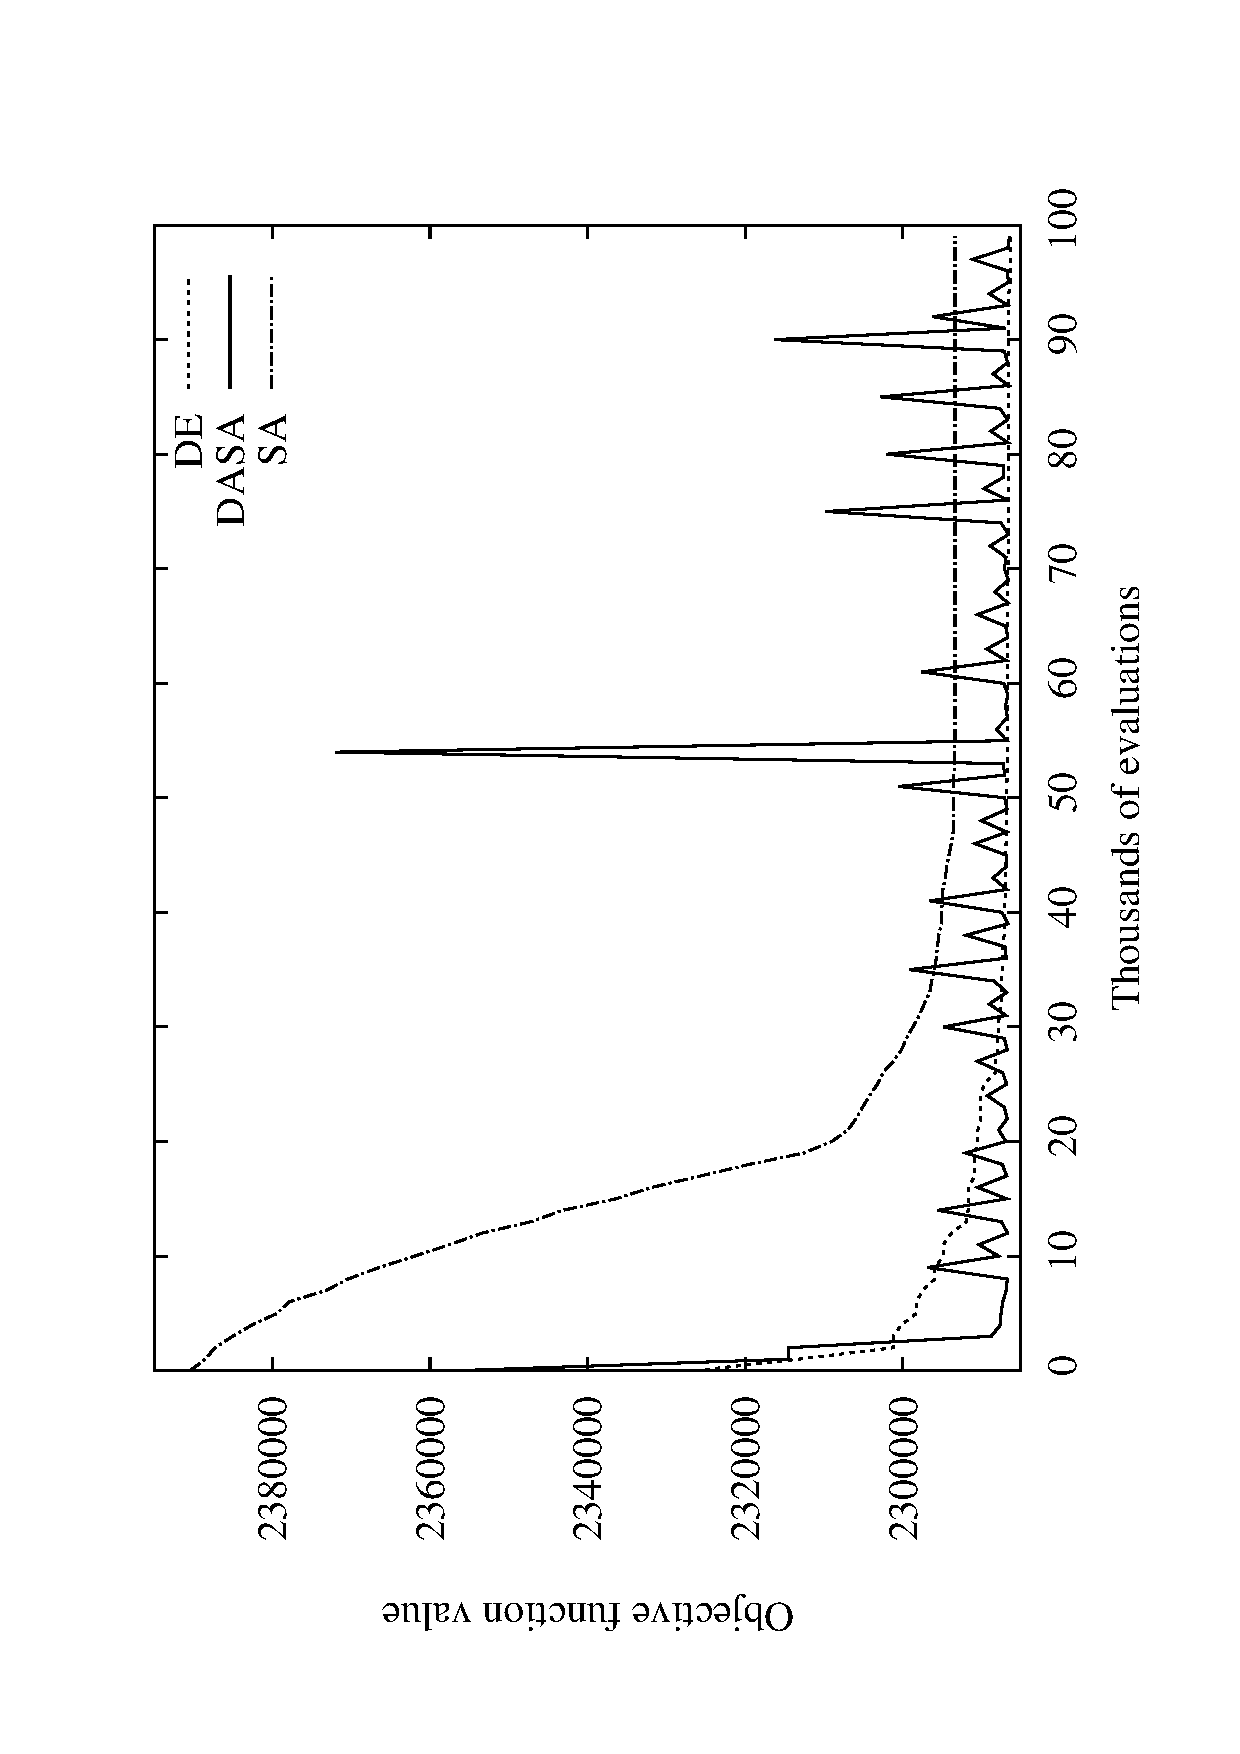
\includegraphics[width=1\columnwidth]{07-experimental_evaluation/img/convergence}\\\vskip -0.3in

\caption{Algorithm convergence for the best obtained results.\label{fig:algorithm_convergence}}
\end{figure}


\begin{table*}
\centering

\caption{Optimization results.\textit{\label{tab:optimization-results}}}


\begin{tabular}{ccccccc}
\toprule 
 & Uncovered area & Covered area, no SHO & Normal SHO area & no SHO$^{\downarrow}$, SHO$^{\uparrow}$ & SHO$^{\downarrow}$, no SHO$^{\uparrow}$ & Total\tabularnewline\addlinespace
\midrule
Before optimization & 63.00 \% & 15.11 \% & 15.73 \% & 1.80 \% & 4.36 \% & 100.00 \%\tabularnewline
\cmidrule{2-7} 
DE solution & 60.23 \% & 16.13 \% & 16.09 \% & 1.47 \% & 6.08 \% & 100.00 \%\tabularnewline
DASA solution & 60.24 \% & 16.16 \% & 16.90 \% & 1.46 \% & 5.24 \% & 100.00 \%\tabularnewline
SA solution & 60.42 \% & 16.55 \% & 15.97 \% & 1.56 \% & 5.50 \% & 100.00 \%\tabularnewline
\cmidrule{2-7} 
DE improvement & +4.40 \% & +6.75 \% & +2.29 \% & +18.33 \% & -39.45 \% & ---\tabularnewline
DASA improvement & +4.38 \% & +6.95 \% & +7.44 \% & +18.88 \% & -20.18 \% & ---\tabularnewline
SA improvement & +4.09 \% & +9.53 \% & +1.52 \% & +13.33 \% & -26.15 \% & ---\tabularnewline
\cmidrule{2-7} 
Avg. improvement & +4.29 \% & +7.74 \% & +3.75 \% & +16.85 \% & -28.59 \% & ---\tabularnewline
\bottomrule
\end{tabular}
\end{table*}


\begin{figure*}
\centering

\begin{minipage}[t]{0.5\textwidth}%
\centering

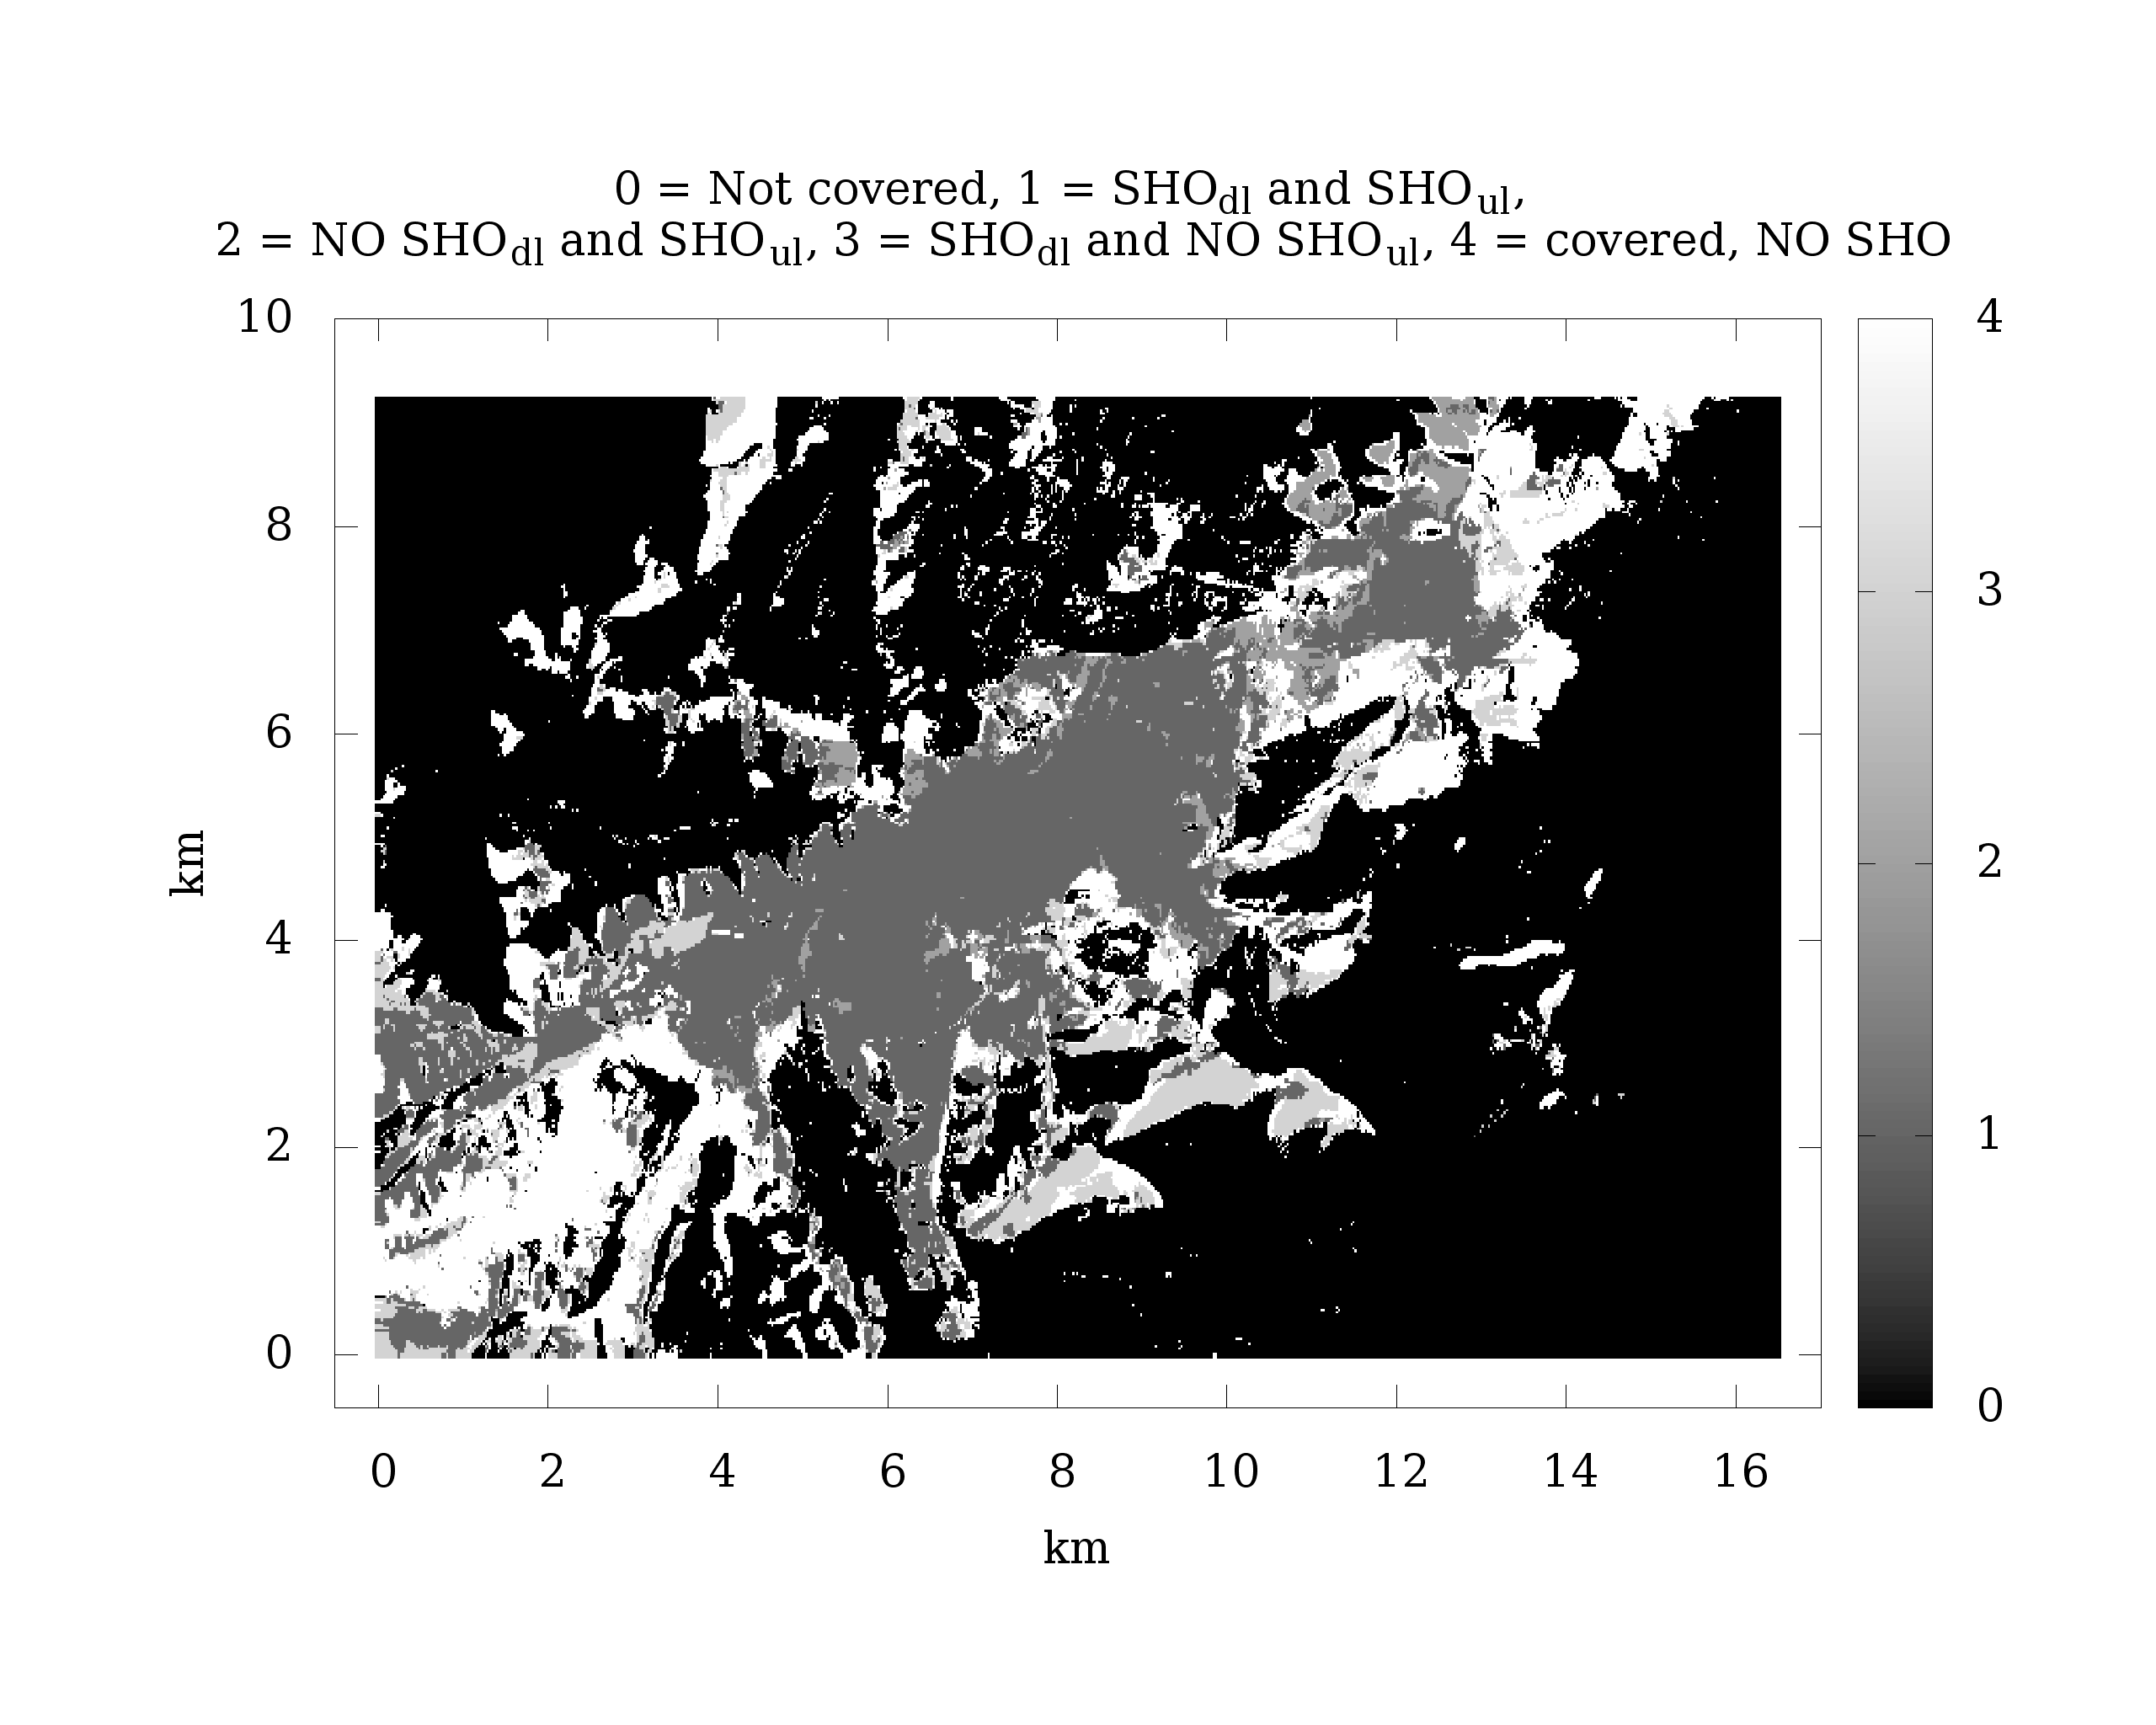
\includegraphics[width=1\textwidth]{07-experimental_evaluation/img/sho_areas_initial}\vskip -0.3in

\caption{Spatial distribution of SHO areas, before optimization.\label{fig:sho_areas_initial}}
%
\end{minipage}\hfill{}%
\begin{minipage}[t]{0.5\textwidth}%
\centering

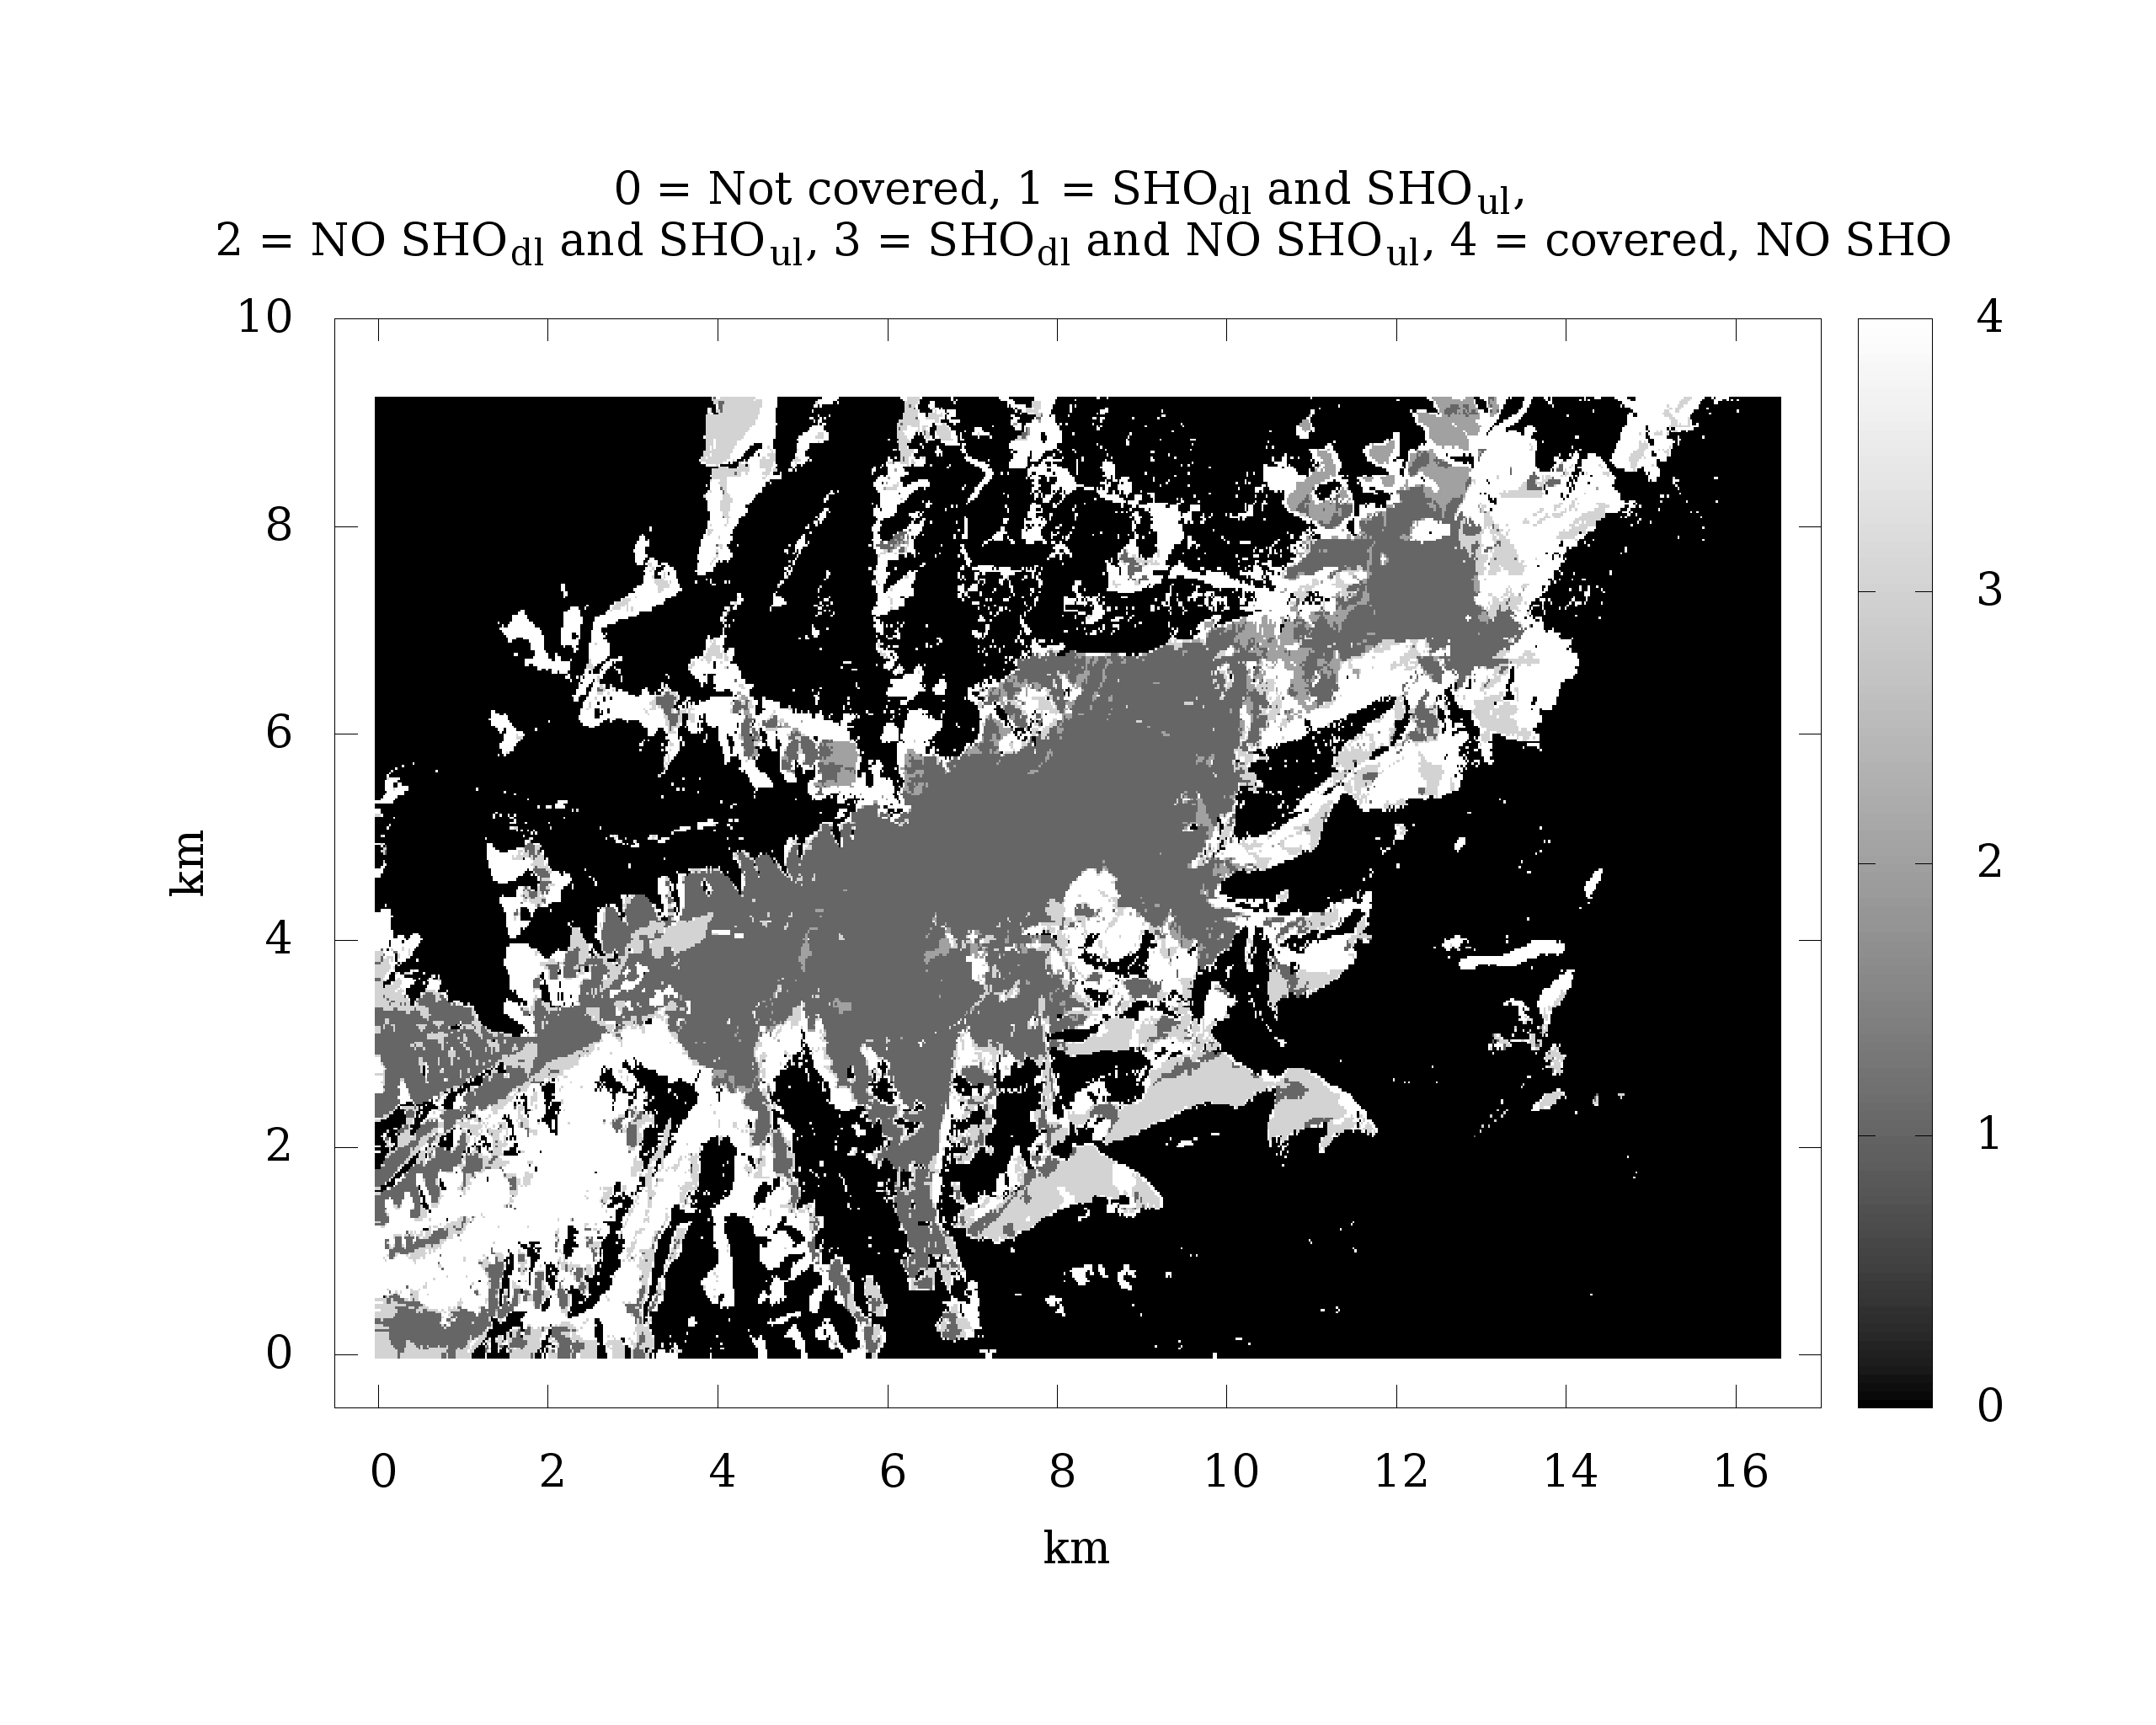
\includegraphics[width=1\textwidth]{07-experimental_evaluation/img/sho_areas_final}\vskip -0.3in

\caption{Spatial distribution of SHO areas, after optimization.\label{fig:sho_areas_final}}
%
\end{minipage}
\end{figure*}


The convergence of the best-recorded run of each of the three algorithms
is shown in Figure \ref{fig:algorithm_convergence}. It is worth mentioning
that every optimization run starts from a different solution, randomly
constructed by picking a CPICH power setting, $p_{i}^{k}$, from every
$P_{i}=\{p_{i}^{1},p_{i}^{2},...,p_{i}^{K}\}$, $1\le k\le|P_{i}|$,
$\forall i\in N$. Notice how fast DASA converges to a good solution.
After a number of evaluations without improvement, DASA resets itself
and continues searching from a new random point within the search
space \cite{korosec2010_DASA}, hence the jagged profile on the graph.
Similarly, DE converges considerably fast, although not as fast as
DASA does. It this case, DE does not reset itself if the current solution
cannot be improved. Despite this, and based on the flat profile the
graph exhibits towards the end of the optimization run, we are confident
that 100,000 evaluations is an adequate stopping criterion for this
algorithm. The last algorithm, SA, slowly converges towards the best
solution found, even though it is not as good as the solutions found
by DE and DASA. 

The three convergence profiles shown in Figure \ref{fig:algorithm_convergence}
give a clearer notion about the way these algorithms explore the search
space of the balancing problem.

Running times of the algorithms are intentionally omitted, since the
implementations used are fundamentally different and therefore not
comparable.


\subsection{Interpretation}

Table \ref{tab:optimization-results} presents the analysis of the
obtained results from the network point of view. After 30 independent
runs of each of the three algorithms, the best results obtained where
evaluated for improvement and decline of each of the measured network
aspects. The results are shown in Table \ref{tab:optimization-results},
where '+' indicates improvement and '-' indicates decline of the given
criteria. We may observe that the measured criteria have been significantly
improved. The only exception is the measure labeled as \textquoteleft{}SHO$^{\downarrow}$,
no SHO$^{\uparrow}$\textquoteleft{}, which shows an expected change,
since it is the optimization aspect with the lowest penalty factor
value.

Coverage has been improved with an average of 4.29\%, whereas the
coverage area where there is no SHO capability has been increased
7.74\% in average. The SHO areas, where this facility is available
in both the downlink and uplink, has also been improved 3.75\% in
average. This particular improvement is interesting from the optimization
point of view, because it had no explicit penalty factor set. Therefore
we understand this enhancement as a consequence of the completeness
of criteria, taken into account in the objective function.

The second most important optimized aspect in the balancing problem
is the proportion of areas with uplink SHO and no SHO in the downlink
(labeled as \textquoteleft{}no SHO$^{\downarrow}$, SHO$^{\uparrow}$\textquoteleft{}
in Table \ref{tab:optimization-results}). This particular condition
has been improved by almost 17\% in average, greatly reducing the
possibility of interference in neighboring cells when serving HSPA
traffic. The last measured aspect takes into account areas with downlink
SHO and no SHO in the uplink (labeled as \textquoteleft{}SHO$^{\downarrow}$,
no SHO$^{\uparrow}$\textquoteleft{} in Table \ref{tab:optimization-results}).
This condition, although it hasn't improved, does not expose the mobile
network to malfunctioning, only to reduced throughput within these
specific areas. However, the reduced throughput is relative, since
there are many cells capable of serving HSDPA data access, as the
downlink SHO condition confirms. For this reason, the serving cell
should not only deliver HSDPA, but should also take care of the user
signaling and power control, received in the uplink. Obviously, this
is only feasible in areas where uplink coverage is guaranteed.

It is worth mentioning that these results were obtained for a working
mobile network with live data. Moreover, the hard constraints imposed
to the optimization process (CPICH power limited within the $\pm$2
dB interval) ensure that the resulting configuration may be immediately
applied to the mobile network. This fact can be contrasted with the
spatial distribution of each of the optimized aspects, before and
after applying the optimization results, as it is shown in Figures
\ref{fig:sho_areas_initial} and \ref{fig:sho_areas_final}.

The lack of any prominent visual change in Figures \ref{fig:sho_areas_initial}
and \ref{fig:sho_areas_final} is a desired consequence of the fine-tuning
procedure the network has been exposed to. Still, the improvements
are present precisely over the areas that are most exposed to malfunctioning
due to unbalanced SHO, e.g. their borders.


\section{Summary \label{sec:Conclusion}}

We have presented the problem of balancing SHO areas in UMTS networks
and characterized some of the consequences unbalanced SHO areas have
on the quality of HSPA services. By using a static network simulator,
based on a state-of-the-art mathematical model, we have located downlink
and uplink SHO areas. Both the mathematical model and the penalty
scores of the objective function have been set according to the configuration
and layout of a real mobile network, deployed in Slovenia by Telekom
Slovenije, d.d.. The balancing problem has been tackled by three optimization
algorithms, namely DE, DASA and SA. To the best of our knowledge,
there is no reference in the literature to a simulation-based approach
to find active SHO areas in the downlink and uplink. Additionally,
as far as we know, the SHO balancing problem, as described in this
paper, has not yet been tackled by any formal optimization method.

All three algorithms were able to improve the given network configuration,
being DE the most successful one. Based on this fact, we may say that
DE was the best suited algorithm for solving our problem. The presented
results confirm that a great proportion of the non-aligned SHO areas,
that were present before the optimization, were corrected, therefore
significantly reducing the possibility of HSPA-service failures within
these areas. Additionally, network coverage has been improved, while
all other essential network services were not altered. 

One of the key advantages of the presented method is that it targets
the optimization of a deployed network, for which the focus is put
on fine-tuning an existing configuration instead of creating complete
new solutions. Furthermore, a deployed network has a great number
of hard-constraints that should be taken into account at the optimization
stage, yet our approach is simple and versatile enough for it to be
used in practically any working UMTS network. Moreover, our model
is applicable for mobile networks in heterogeneous environments, because
it imposes no restrictions regarding cell layout or radio propagation
characteristics.

To further improve the presented results, dynamic effects, such as
fast power control, should be included in the simulations, since it
is a valuable element of a WCDMA mobile system. Another extension
of the current work is to incorporate antenna tilt as an additional
objective of the optimization process. This should certainly include
experimentation with models and algorithms that support multiobjective
optimization.
